% $Header$

\documentclass{beamer}
% common for paper and presentation

%%-- My stuff

\usepackage{pdfpages}[interpolate=false]
\usepackage{amsmath,amsfonts,amsthm}
\usepackage{mathtools,bm}
\usepackage{listings,color}
\usepackage{tikz,float}
\usepackage[font=small]{caption}
\usetikzlibrary{arrows,snakes,backgrounds}
%funk for externalizing graphics...
%\pgfrealjobname{thesis}


\newcommand{\lstVecMat}{\lstinputlisting[firstline=10, firstnumber=10, lastline=11]{../cpp/include/common.h}}
\newcommand{\lstVPoly}{\lstinputlisting[firstline=13, firstnumber=13, lastline=16]{../cpp/include/common.h}}
\newcommand{\lstD}{\lstinputlisting[firstline=20, firstnumber=20, lastline=20]{../cpp/include/common.h}}
\newcommand{\lstIstream}{\lstinputlisting[firstline=22, firstnumber=22, lastline=25]{../cpp/include/common.h}}
\newcommand{\lstOstream}{\lstinputlisting[firstline=26, firstnumber=26, lastline=29]{../cpp/include/common.h}}
\newcommand{\lstInputError}{\lstinputlisting[firstline=30, firstnumber=30, lastline=30]{../cpp/include/common.h}}
\newcommand{\lstUsage}{\lstinputlisting[firstline=36, firstnumber=36, lastline=36]{../cpp/include/common.h}}
\newcommand{\lstTranspose}{\lstinputlisting[firstline=41, firstnumber=41, lastline=41]{../cpp/include/common.h}}
\newcommand{\lstProjectM}{\lstinputlisting[firstline=44, firstnumber=44, lastline=44]{../cpp/include/common.h}}
\newcommand{\lstCheckEmpty}{\lstinputlisting[firstline=129, firstnumber=129, lastline=131]{../cpp/src/common.cpp}}
\newcommand{\lstFME}{\lstinputlisting[firstline=166, firstnumber=166, lastline=183]{../cpp/src/common.cpp}}
\newcommand{\lstFMEPart}{\lstinputlisting[firstline=169, firstnumber=169, lastline=172]{../cpp/src/common.cpp}}
\newcommand{\lstFMEMove}{\lstinputlisting[firstline=174, firstnumber=174, lastline=174]{../cpp/src/common.cpp}}
\newcommand{\lstFMEConvolute}{\lstinputlisting[firstline=176, firstnumber=176, lastline=181]{../cpp/src/common.cpp}}
\newcommand{\lstLiftHcone}{\lstinputlisting[firstline=13, firstnumber=13, lastline=13]{../cpp/include/hcone.h}}
\newcommand{\lstIntersectVCone}{\lstinputlisting[firstline=53, firstnumber=53, lastline=59]{../cpp/src/hcone.cpp}}
\newcommand{\lstHconeToVcone}{\lstinputlisting[firstline=63, firstnumber=63, lastline=69]{../cpp/src/hcone.cpp}}
\newcommand{\lstLiftVcone}{\lstinputlisting[firstline=9, firstnumber=9, lastline=9]{../cpp/include/vcone.h}}
\newcommand{\lstProjectHCone}{\lstinputlisting[firstline=51, firstnumber=51, lastline=57]{../cpp/src/vcone.cpp}}
\newcommand{\lstVconeToHcone}{\lstinputlisting[firstline=61, firstnumber=61, lastline=67]{../cpp/src/vcone.cpp}}
\newcommand{\lstProjectZero}{\lstinputlisting[firstline=12, firstnumber=12, lastline=16]{../cpp/src/polyhedra.cpp}}
\newcommand{\lstNormalizeP}{\lstinputlisting[firstline=20, firstnumber=20, lastline=30]{../cpp/src/polyhedra.cpp}}
\newcommand{\lstHpolyToHCone}{\lstinputlisting[firstline=34, firstnumber=34, lastline=42]{../cpp/src/polyhedra.cpp}}
\newcommand{\lstHconeToHPoly}{\lstinputlisting[firstline=46, firstnumber=46, lastline=54]{../cpp/src/polyhedra.cpp}}
\newcommand{\lstVpolyToVCone}{\lstinputlisting[firstline=59, firstnumber=59, lastline=74]{../cpp/src/polyhedra.cpp}}
\newcommand{\lstVconeToVPoly}{\lstinputlisting[firstline=78, firstnumber=78, lastline=92]{../cpp/src/polyhedra.cpp}}
\newcommand{\lstHpolyToVPoly}{\lstinputlisting[firstline=96, firstnumber=96, lastline=98]{../cpp/src/polyhedra.cpp}}
\newcommand{\lstVpolyToHPoly}{\lstinputlisting[firstline=100, firstnumber=100, lastline=102]{../cpp/src/polyhedra.cpp}}


\renewcommand{\vec}[1]{\mathbf{#1}}
\newcommand{\set}[1]{\left\{#1\right\}}
\DeclareMathOperator{\cone}{cone}
\DeclareMathOperator{\conv}{conv}
\DeclareMathOperator{\VLift}{T_V}
\DeclareMathOperator{\HLift}{T_H}
\newcommand{\ip}[2]{\left\langle #1, #2 \right\rangle}

%special letters
\newcommand{\R}{\mathbb{R}}
\newcommand{\0}{\vec{0}}
\newcommand{\1}{\vec{1}}
\renewcommand{\r}{\vec{r}}
\renewcommand{\u}{\vec{u}}
\newcommand{\x}{\vec{x}}
\newcommand{\y}{\vec{y}}
\newcommand{\z}{\vec{z}}
\newcommand{\e}{\vec{e}}
\newcommand{\w}{\vec{w}}
\renewcommand{\t}{\vec{t}}
\renewcommand{\v}{\vec{v}}
\renewcommand{\b}{\vec{b}}
\newcommand{\faij}{\forall i\in P,\forall j \in N}
\newcommand{\blambda}{\bm{\lambda}}
\newcommand{\bsigma}{\bm{\sigma}}
\newcommand{\bmu}{\bm{\mu}}

%symbols
\newcommand{\st}{\;|\;}
\newcommand{\St}{\;\Big|\;}

%constants
\newcommand{\Udim}{p}
\newcommand{\Vdim}{n}
\newcommand{\Adim}{m}
\newcommand{\mspaceA}{\R^{{\Adim}\times d}}
\newcommand{\mspaceB}{\R^{m_1\times (d+\Udim)}}
\newcommand{\mspaceC}{\R^{m_2\times (d+\Udim)}}

%matrices and vectors with domain
\newcommand{\bv}{\b \in \R^{\Adim}}
\newcommand{\tv}{\t \in \R^{\Udim}}
\renewcommand{\l}{\bm{\lambda}}
\newcommand{\lv}{\l \in \R^{\Vdim}}
\newcommand{\yv}{\y \in \R^{d+1}}
\newcommand{\xv}{\x \in \R^d}
\newcommand{\mV}{V \in \R^{d\times \Vdim}}
\newcommand{\mU}{U \in \R^{d\times \Udim}}
\newcommand{\mA}{A \in \mspaceA}
\newcommand{\mB}{B \in \mspaceB}
\newcommand{\mC}{B' \in \mspaceC}
\newcommand{\xt}{\pmb  \x\\ \t\pme }
\newcommand{\xw}{\pmb  \x\\ \w\pme }
\newcommand{\xAx}{\pmb \x\\ A\x\pme }
\newcommand{\xz}{\pmb  \x\\ \0\pme }
\newcommand{\xx}{\pmb  x_0\\ \x\pme }
\newcommand{\sxx}{\psmb  x_0\\ \x\psme }
\newcommand{\onex}{\pmb 1\\ \x\pme }
\newcommand{\zw}{\pmb  \0\\ \w\pme }
\newcommand{\eAj}{\pmb \e_j\\ A^j\pme }
\newcommand{\neAj}{\pmb -\e_j\\ -A^j\pme }
\newcommand{\ee}{\pmb  \0 \\ 1 \pme }
\newcommand{\zei}{\pmb \0 \\ \e_i \pme }
\newcommand{\lcone}{\pmb  \0 & \vec{1} \\ U & V \pme }
\newcommand{\xjp}{x_j^+}
\newcommand{\xjm}{x_j^-}
\newcommand{\Yi}{Y^i_{k}}
\newcommand{\Yj}{Y^j_{k}}
\newcommand{\Yl}{Y^l_{k}}
\newcommand{\Uiz}{U^i_{0}}
\newcommand{\Ujz}{U^j_{0}}
\newcommand{\Ulz}{U^l_{0}}
\newcommand{\Bik}{B^k_i}
\newcommand{\Bjk}{B^k_j}
\newcommand{\Blk}{B^k_l}

%sums
\newcommand{\tusum}{\sum_{1\leq j \leq \Udim}t_j U^j}
\newcommand{\lvsum}{\sum_{1\leq j \leq \Vdim}\lambda_j V^j}
\newcommand{\lsum}{\sum_{1\leq j \leq \Vdim}\lambda_j}
\newcommand{\jsum}{\sum_{1\leq j \leq d}}
\newcommand{\isum}{\sum_{1\leq i \leq n}}
\newcommand{\Psum}{\sum_{i\in P}}
\newcommand{\Nsum}{\sum_{j\in N}}
\newcommand{\Zsum}{\sum_{l\in Z}}
\newcommand{\NPsum}{\sum_{\substack{i\in P \\ j\in N}}}
\newcommand{\isconv}{\lambda_j \geq 0 \lsum = 1}
\newcommand{\sumi}{\sum\nolimits_i}
\newcommand{\sumj}{\sum\nolimits_j}

% Polyhedra
\newcommand{\HC}[1]{\set{\x\st #1\x\leq\0}}
\newcommand{\HP}[2]{\set{\x\st #1\x\leq #2}}
\newcommand{\VP}[2]{\cone(#1) + \conv(#2)}
\newcommand{\LHC}{\set{\xx\St\big[-\vec{b}|A\big]\xx\leq\0}}
\newcommand{\hpxz}{\set{\xx\St x_0 = 1}}
\newcommand{\shpxz}{\set{\sxx\st x_0 = 1}}

\usepackage{thmtools,cleveref}

%text macros
\newcommand{\MWT}{Minkowski-Weyl Theorem}
\newcommand{\texteq}[2]{\begin{equation}\text{#1}\label{#2}\end{equation}}
\newcommand{\LI}{linear-independent}

%code stuff
\newcommand{\cppSourceDir}{../../cpp}
%%
\newcommand{\smallstack}[2]{\left(\begin{smallmatrix}#1 \\ #2\end{smallmatrix}\right)}

\newcommand{\lsti}[1]{\lstinline!#1!}
\newcommand{\filename}[1]{\texttt{#1}}
\newcommand{\mli}[1]{\text{\lsti{#1}}}
\newcommand{\norm}[1]{\left|\left|#1\right|\right|}
\renewcommand{\pmb}{\begin{pmatrix*}[r]}
\newcommand{\pme}{\end{pmatrix*}}
\newcommand{\psmb}{\begin{psmallmatrix*}[r]}
\newcommand{\psme}{\end{psmallmatrix*}}

\lstset{
	language=C++,
	backgroundcolor=\color[rgb]{.9,.9,.9},
	basicstyle=\small\tt,
	keywordstyle=\color[rgb]{0,.2,1},
	commentstyle=\color[rgb]{0,.6,.2},
	numbers=left,
	showstringspaces=false
}

%max bound
\newcommand{\MX}{10}
%draw the grid 
\newcommand{\drawGrid}{
	\clip (-1,-1) rectangle (4,4);
	\draw[style=help lines] (-\MX,-\MX) grid (\MX,\MX);
	\draw[style=very thick] (0,\MX) -- (0,-\MX);
	\draw[style=very thick] (\MX,0) -- (-\MX,0);
}
%various constants
\newcommand{\lowSlopeX}{2}
\newcommand{\lowSlopeY}{1}
\pgfmathsetmacro{\lowSlope}{\lowSlopeY / \lowSlopeX}
\newcommand{\highSlopeX}{1}
\newcommand{\highSlopeY}{2}
\pgfmathsetmacro{\highSlope}{\highSlopeY / \highSlopeX}
\newcommand{\myslope}{0}
\newcommand{\genLen}{2}
\newcommand{\lowVertX}{2}
\newcommand{\highVertX}{1.5}
\newcommand{\vertexRadius}{.08}
\newcommand{\origin}{(0,0)}
%
\tikzstyle ConeStyle=[fill, color=gray, style=semitransparent]
\tikzstyle GeneratorInd=[style=dotted, thick, color=blue]
\tikzstyle GeneratorSty=[->, style=thick, color=blue]
%
%draw the constraints: #1 - slope, #2 lt or rt
\newcommand{\getHatchLine}[3]{
	\renewcommand{\myslope}{#1}
	\pgfmathsetmacro{\myAngle}{atan{\myslope}}
	\draw[style=thick, color=blue] #3 -- +(\myAngle:-\MX);
	\draw[style=thick, color=blue] #3 -- +(\myAngle:\MX);
	\pgfmathsetmacro{\myHatchAngle}{\myAngle + #2*90}
	\foreach \x in {-\MX, -9.5, ..., \MX} {
			\draw[style=thick, color=blue] #3 ++(\myAngle:\x) -- +(\myHatchAngle:.15);
		}
}
\newcommand{\drawGenerator}[1]{
	\draw[style=GeneratorSty] \origin -- (#1:\genLen);
}
\newcommand{\drawSegment}[2]{
	\draw[fill, color=blue] #1 circle (\vertexRadius);
	\draw[fill, color=blue] #2 circle (\vertexRadius);
	\draw[style=thick, color=blue] #1 -- #2;
}
%draws the cone: #1 - low slope, #2 - high slope
\newcommand{\coneConstraints}[2]{
	\getHatchLine{#1}{1}{\origin};
	\getHatchLine{#2}{-1}{\origin};
}
%draws the cone: #1 - low slope, #2 - high slope, #3 vertex
\newcommand{\polyConstraints}[5]{
	\getHatchLine{#1}{1}{\origin};
	\getHatchLine{#2}{-1}{\origin};
	\getHatchLine{#4}{#5}{#3};
}
%draws the generators
\newcommand{\coneGenerators}[2]{
	\drawGenerator{\lowDir};
	\drawGenerator{\highDir};
	\draw[style=GeneratorInd] (\lowDir:\genLen) arc (\lowDir:\highDir:\genLen);
}
%V-Polyhedra: low, high, vert
\newcommand{\polyGenerators}[3]{
	\drawGenerator{\highDir};
	\draw[style=GeneratorInd] (\highDir:\genLen) -- ++ #3;
	\drawSegment{\origin}{\lowVert};
}
%V-Polytope
\newcommand{\vPolytope}{
	\drawSegment{\origin}{\lowVert}
	\drawSegment{\origin}{\highVert}
	\drawSegment{\lowVert}{\highVert}
}
%H-Polytope
\newcommand{\hPolytope}{
	\polyConstraints{\lowSlope}{\highSlope}{\lowVert}{-4.0}{-1}
}
%draws the h-constraints
\newcommand{\drawCone}{
	\draw[style=ConeStyle] \origin -- (\MX,\lowY) -- (\MX,\highY);
}
%draws the polyhedra
\newcommand{\drawPolyhedra}{
	\draw[style=ConeStyle] \origin -- \lowVert -- ++(\MX,\highY) -- (\MX,\highY);
}
%draws the polytope
\newcommand{\drawPolytope}{
	\draw[style=ConeStyle] \origin -- \lowVert -- \highVert;
}

%
\pgfmathsetmacro{\lowY}{\MX * \lowSlope}
\pgfmathsetmacro{\highY}{\MX * \highSlope}
\pgfmathsetmacro{\lowVertY}{\lowVertX * \lowSlope}
\pgfmathsetmacro{\highVertY}{\highVertX * \highSlope}
\pgfmathsetmacro{\lowDir}{atan{\lowSlope}}
\pgfmathsetmacro{\highDir}{atan{\highSlope}}

\newcommand{\lowVert}{(\lowVertX,\lowVertY)}
\newcommand{\highVert}{(\highVertX,\highVertY)}

\newcommand{\svec}[2]{\begin{bmatrix*}[r] #1 \\ #2 \end{bmatrix*}}

%H-Cone
\newcommand{\drawHCone}{
	\begin{figure}[h]
		\centering
		\begin{tikzpicture}
			\drawGrid
			\drawCone
			\coneConstraints{\lowSlope}{\highSlope}
		\end{tikzpicture}
		\caption[]{H-Cone: $\pmb
				-\highSlopeY & \highSlopeX \\
				\lowSlopeY & -\lowSlopeX
				\pme \pmb x \\ y \pme \leq \pmb 0 \\ 0 \pme$}
	\end{figure}
}

%V-Cone
\newcommand{\drawVCone}{
	\begin{figure}[h]
		\centering
		\begin{tikzpicture}
			\drawGrid
			\drawCone
			\coneGenerators{\lowSlope}{\highSlope}
		\end{tikzpicture}
		\caption[]{V-Cone: $\cone\left(
				\svec{\highSlopeX}{\highSlopeY},
				\svec{\lowSlopeX}{\lowSlopeY}\right)$}
	\end{figure}
}

%H-Polyhedra
\newcommand{\drawHPoly}{
	\begin{figure}[h]
		\centering
		\begin{tikzpicture}
			\drawGrid
			\drawPolyhedra
			\polyConstraints{\lowSlope}{\highSlope}{\lowVert}{\highSlope}{1}
		\end{tikzpicture}
		\caption[]{H-Polyhedra: $\pmb
				-\highSlopeY & \highSlopeX \\
				\lowSlopeY & -\lowSlopeX \\
				\highSlopeY & -\highSlopeX
				\pme \pmb x \\ y \pme \leq \pmb 0 \\ 0 \\ 3 \pme$}
	\end{figure}
}

%V-Polyhedra
\newcommand{\drawVPoly}{
	\begin{figure}[h]
		\centering
		\begin{tikzpicture}
			\drawGrid
			\drawPolyhedra
			\polyGenerators{\lowSlope}{\highSlope}{\lowVert}
		\end{tikzpicture}
		\caption[]{V-Polyhedra: $\cone\left(
				\svec{\highSlopeX}{\highSlopeY}\right) +
				\conv\left(\svec{0}{0}, \svec{\lowVertX}{1}\right)$}
	\end{figure}
}

%H-Polytope
\newcommand{\drawHPolytope}{
	\begin{figure}[h]
		\centering
		\begin{tikzpicture}
			\drawGrid
			\drawPolytope
			\hPolytope
		\end{tikzpicture}
		\caption[]{H-Polytope: $\pmb
				-\highSlopeY & \highSlopeX \\
				\lowSlopeY & -\lowSlopeX \\
				4 & 1
				\pme \pmb x \\ y \pme \leq \pmb 0 \\ 0 \\ 9 \pme$}
	\end{figure}
}

%V-Polytope
\newcommand{\drawVPolytope}{
	\begin{figure}[h]
		\centering
		\begin{tikzpicture}
			\drawGrid
			\drawPolytope
			\vPolytope
		\end{tikzpicture}
		\caption[]{V-Polytope: $\conv\left(
				\svec{0}{0},
				\svec{\lowVertX}{1},
				\svec{1.5}{3}
				\right)$}
	\end{figure}
}

%Not Full Dim
\newcommand{\drawNotFullDim}{
	\begin{figure}[h]
		\centering
		\begin{tikzpicture}
			\drawGrid
			\getHatchLine{\highSlope}{1}{\origin};
			\getHatchLine{\highSlope}{-1}{\origin};
			\getHatchLine{-1}{1}{\origin};
			\getHatchLine{0.}{1}{\origin};
		\end{tikzpicture}
		\caption[]{H-Cone, not full-dimensional: \\
			$\pmb -2 & 1 \\ 2 & -1 \\ -1 & -1 \\ 0 & -1 \pme \pmb x \\ y \pme
				\leq \pmb 0 \\ 0 \\ 0 \\ 0 \pme$ }
	\end{figure}
}

%Not Pointed
\newcommand{\drawNotPointed}{
	\begin{figure}[h]
		\centering
		\begin{tikzpicture}
			\clip (-3,-3) rectangle (3,3);
			\draw[style=help lines] (-\MX,-\MX) grid (\MX,\MX);
			\draw[style=very thick] (0,\MX) -- (0,-\MX);
			\draw[style=very thick] (\MX,0) -- (-\MX,0);
			\draw[style=GeneratorSty] \origin -- (135:2.);
			\draw[style=GeneratorSty] \origin -- (-45:2.);
			\draw[style=GeneratorSty] \origin -- (0,2);
			\draw[style=GeneratorSty] \origin -- (2,0);
			\draw[style=ConeStyle] \origin -- (-\MX,\MX) -- (\MX,\MX) -- (\MX,-\MX);
		\end{tikzpicture}
		\caption[]{V-Cone, not pointed: $\cone\left(
				\svec{\highSlopeX}{\highSlopeY},
				\svec{\lowSlopeX}{\lowSlopeY},
				\svec{0}{2},
				\svec{2}{0}
				\right)$}
	\end{figure}
}



% This file is a solution template for:

% - Talk at a conference/colloquium.
% - Talk length is about 20min.
% - Style is ornate.



% Copyright 2004 by Till Tantau <tantau@users.sourceforge.net>.
%
% In principle, this file can be redistributed and/or modified under
% the terms of the GNU Public License, version 2.
%
% However, this file is supposed to be a template to be modified
% for your own needs. For this reason, if you use this file as a
% template and not specifically distribute it as part of a another
% package/program, I grant the extra permission to freely copy and
% modify this file as you see fit and even to delete this copyright
% notice. 


\mode<presentation>
{
	\usetheme{Warsaw}
	% or ...

	\setbeamercovered{transparent}
	% or whatever (possibly just delete it)
}


\usepackage[english]{babel}
% or whatever

\usepackage[latin1]{inputenc}
% or whatever

\usepackage{times}
\usepackage[T1]{fontenc}
% Or whatever. Note that the encoding and the font should match. If T1
% does not look nice, try deleting the line with the fontenc.


\title % (optional, use only with long paper titles)
{The \MWT}

%\subtitle
%{Include Only If Paper Has a Subtitle}

\author % (optional, use only with lots of authors)
{Nathan Chappell\inst{1}}
% - Give the names in the same order as the appear in the paper.
% - Use the \inst{?} command only if the authors have different
%   affiliation.

\institute % (optional, but mostly needed)
{
	\inst{1}%
	Charles University\\
	Faculty of Mathematics and Physics
}
% - Use the \inst command only if there are several affiliations.
% - Keep it simple, no one is interested in your street address.

\date % (optional, should be abbreviation of conference name)
{Defense of Bachelor's Thesis, 2019}
% - Either use conference name or its abbreviation.
% - Not really informative to the audience, more for people (including
%   yourself) who are reading the slides online

%\subject{Theoretical Computer Science}
% This is only inserted into the PDF information catalog. Can be left
% out. 



% If you have a file called "university-logo-filename.xxx", where xxx
% is a graphic format that can be processed by latex or pdflatex,
% resp., then you can add a logo as follows:

% \pgfdeclareimage[height=0.5cm]{university-logo}{university-logo-filename}
% \logo{\pgfuseimage{university-logo}}



% Delete this, if you do not want the table of contents to pop up at
% the beginning of each subsection:
\AtBeginSubsection[]
{
	\begin{frame}<beamer>{Outline}
		\tableofcontents[currentsection,currentsubsection]
	\end{frame}
}


% If you wish to uncover everything in a step-wise fashion, uncomment
% the following command: 

%\beamerdefaultoverlayspecification{<+->}


\begin{document}

\begin{frame}
	\titlepage
\end{frame}

\begin{frame}{Outline}
	\tableofcontents
	% You might wish to add the option [pausesections]
\end{frame}


% Structuring a talk is a difficult task and the following structure
% may not be suitable. Here are some rules that apply for this
% solution: 

% - Exactly two or three sections (other than the summary).
% - At *most* three subsections per section.
% - Talk about 30s to 2min per frame. So there should be between about
%   15 and 30 frames, all told.

% - A conference audience is likely to know very little of what you
%   are going to talk about. So *simplify*!
% - In a 20min talk, getting the main ideas across is hard
%   enough. Leave out details, even if it means being less precise than
%   you think necessary.
% - If you omit details that are vital to the proof/implementation,
%   just say so once. Everybody will be happy with that.

\section{Theorem}

\subsection{Definitions and Statement}
%
%\begin{frame}{V/H Polyhedra/Cones}
%  % - A title should summarize the slide in an understandable fashion
%  %   for anyone how does not follow everything on the slide itself.
%
%  \begin{itemize}
%  \item V-Cone: non-negative linear combinations of some set \\
%          $\{U\t : \t \geq \0\}$
%  \item V-Polytope: convex combinations of some set \\
%          $\{V\blambda : \blambda \geq \0, \1^T\blambda = 1\}$
%  \item V-Polyhedron: Minkowski Sum of V-Cone and V-Polytope \\
%          $\{U\t + V\blambda : \t,\blambda \geq \0, \1^T\blambda = 1\}$
%  \item H-Cone: solutions to system of linear inequalities \\
%          $\{\x : A\x \leq \0 \}$
%  \item H-Polyhedra: solutions to system of linear inequalities \\
%          $\{\x : A\x \leq \vec{b} \}$
%  \end{itemize}
%\end{frame}

%my macros
\newcommand{\UCone}{\{U\t \st \t \geq \0\}}
\newcommand{\TUCone}{\pmb \0 & -I \\ I & -U \\ -I & U \pme}

\begin{frame}{V/H Polyhedra/Cones}
	% - A title should summarize the slide in an understandable fashion
	%   for anyone how does not follow everything on the slide itself.

	Let $U \in \R^{d\times l},\, V \in \R^{d\times m},\, A \in \R^{m\times d}$
	\begin{itemize}
		\item V-Cone:\\ $\UCone \;\equiv\; \cone(U)$
		\item V-Polytope:\\ $\{V\blambda \st \blambda \geq \0, \1^T\blambda = 1\} \;\equiv\; \conv(V)$
		\item V-Polyhedron:\\ $\{U\t + V\blambda \st \t,\blambda \geq \0, \1^T\blambda = 1\} \;\equiv\; \cone(U) + \conv(V)$
		\item H-Cone:\\ $\{\x \st A\x \leq \0 \}$
		\item H-Polyhedron:\\ $\{\x \st A\x \leq \vec{b} \}$
	\end{itemize}
\end{frame}

\begin{frame}{\MWT}
	\begin{itemize}
		\item General Statement: \\
		      V-Polyhedra and H-Polyhedra are the same things
		      \pause
		\item For Cones: \\
		      V-Cones and H-Cones are the same things
		      \pause
	\end{itemize}
	First, the proof is done for cones, then polyhedra are reduced to cones.
\end{frame}


\subsection{Proof of the theorem}

\begin{frame}{V-Cones are H-Cones}
	Basic idea:
	\begin{itemize}
		\item rewrite V-Cone as a projection of an H-Cone
		\item show that a projection of an H-Cone is an H-Cone
	\end{itemize}
\end{frame}

\newcommand{\myalignw}{2.2cm}
\def\myialign[#1]#2{\makebox[\myalignw][l]{#1} \;#2\;}

\begin{frame}[t]{V-Cones are H-Cones}{Lifting the V-Cone}
	Say we are given $\UCone\ldots$
	\medskip
	\begin{itemize}
		\only<1>{\item First, the non-negativity constraint}
		      \only<2-7>{\item \myialign[$\t \geq \0$]{$\Leftrightarrow$}
		      $\pmb \0 & -I\pme \xt \leq \0$}
		      \only<3>{\item Next, capture the points}
		      \only<4-7>{\item \myialign[$\x = U\t$]{$\Leftrightarrow$}
		      $\pmb I & -U \\ -I & U \pme \xt \leq \0$}
		      \only<5>{\item Finally, project the combined constraints}
		      \only<6-7>{\item \myialign[$\UCone$]{$=$}
		      $\left\{\x \St \TUCone \xt \leq \0 \right\}$}
	\end{itemize}
	\only<7>{The final expression is a projection of an H-Cone}
\end{frame}

\begin{frame}{V-Cones are H-Cones}{Projecting an H-Cone}
	We project an H-Cone one coordinate at a time with
	\alert{Fourier-Motzkin Elimination}
	\begin{itemize}
		\item<2-> Observation:\\[5pt]
		      $\pmb A & \0 \pme \xt \leq \0 \Leftrightarrow A\x \leq \0$
		\item<3-> Therefore: \\[5pt]
		      $\left\{\x \St \pmb A & \0 \pme \xt \leq \0\right\} =
			      \left\{ \x \st A\x \leq \0 \right\}$
		\item<4-> So, projecting $\0$ columns is easy.
	\end{itemize}
\end{frame}

\begin{frame}{V-Cones are H-Cones}{Fourier-Motzkin Elimination}
	Suppose we are projecting column $k$ from $A\x\leq\0$.
	\begin{itemize}
		\item<2-> First, partition the rows as follows:\\
		      $Z$: rows with $k$-th column $0$ \\
		      $P$: rows with $k$-th column positive\\
		      $N$: rows with $k$-th column negative
		\item<3-> Create a new matrix $A'$ with rows as follows: \\[5pt]
		      $\begin{cases}
				      A_z                   & A_z \in Z            \\
				      A_p^k A_n - A_n^k A_p & A_n \in N, A_p \in P
			      \end{cases}$
		\item<4-> You can show:\\
		      $(\exists t)\,A(\x+t\e_k) \leq \0 \Leftrightarrow A'\x\leq\0$
	\end{itemize}
\end{frame}

\begin{frame}{H-Cones are V-Cones}
	Basic idea:
	\begin{itemize}
		\item rewrite V-Cone as a projection of intersection of an H-Cone with hyperplanes
		\item show that a intersection of a V-Cone with a hyperplane is a V-Cone
		\item projecting V-Cones is easy
	\end{itemize}
\end{frame}

\begin{frame}[t]{H-Cones are V-Cones}{Lifting the H-Cone}
	Say we are given $\HC{A}\ldots$
	\medskip
	\begin{itemize}
		\only<1>{\item First, take up the slack}
		      \only<2-7>{\item \myialign[$A\x\leq\0$]{$\Leftrightarrow$}
		      $\exists \w\geq\0 \st A\x + \w = \0$}
		      \only<3>{\item Next, capture the points}
		      \only<4-7>{\item
		      \myialign[$A\x + \w = \0$]{$\Leftrightarrow$}
		      $\pmb \x \\ A\x \pme + \pmb \0 \\ \w \pme = \pmb \x \\ \0 \pme$}
		      \only<5>{\item Finally, split the positive/negative contributions:}
		      \only<6-7>{\item \myialign[$A\x\leq\0$]{$\Leftrightarrow$}
		      $\xz \in \cone\pmb I & -I & \0 \\ A & -A & I \pme$}
	\end{itemize}
	\only<7>{The final expression is a intersection of a V-Cone with some hyperplanes}
\end{frame}

\begin{frame}[t]{H-Cones are V-Cones}{Intersecting a V-Cone}
	We intersect a V-Cone one coordinate at a time with
	\alert{Dual-Fourier-Motzkin Elimination}
	\begin{itemize}
		\item<2-> We need to characterize elements of $\cone(U)$ with the $k$-th element $0$.
		      \only<3>{\item We use the following algebraic trick$\ldots$}
		      \only<4-6>{
		\item<4-> Suppose that $\x_i, \x_j \in \cone(U)$, $x_j^k < 0 < x_i^k$, $\sum_i x_i^k + \sum_j x_j^k = 0$, and let $1/\sigma := \sum_i x_i^k = -\sum_j x_j^k$.
		\item<5-> We can rewrite $\sum_j \x_j + \sum_i \x_i = \sigma \sum_{i,j} x_i^k \x_j - x_j^k \x_i$
		\item<6-> Note that: $x_i^k\x_j - x_j^k\x_i \in \cone(U) \cap \{\x \st x^k = 0\}$
		      }
	\end{itemize}
\end{frame}

\begin{frame}{H-Cones are V-Cones}{Fourier-Motzkin Elimination}
	Suppose we are intersecting $\set{x_k = 0}$ with $\cone(U)$.
	\begin{itemize}
		\item<2-> First, partition the columns as follows:\\
		      $Z$: columns with $k$-th row $0$ \\
		      $P$: columns with $k$-th row positive\\
		      $N$: columns with $k$-th row negative
		\item<3-> Create a new matrix $U'$ with columns as follows: \\[5pt]
		      $\begin{cases}
				      \x_z                      & \x_z \in Z             \\
				      \x_p^k \x_n - \x_n^k \x_p & \x_n \in N, \x_p \in P
			      \end{cases}$
		\item<4-> You can show:\\
		      $\y \in \cone(U), y^k = 0 \Leftrightarrow \y \in \cone(U')$
	\end{itemize}
\end{frame}

\begin{frame}{Reducing Polyhedra to Cones}
	\begin{itemize}
		\item For H-Polyhedra, move constraints to column $0$ and set that coordinate to $1$
		      \pause
		\item $\HP{A}{\vec{b}} = \LHC \cap \hpxz$
		      \pause
		\item For V-Polyhedra, use an intersection to enforce convex combinations
		      \pause
		\item $\VP{U}{V} = \Pi\left(\cone\pmb \0 & \1 \\ U & V \pme \cap \hpxz\right)$
	\end{itemize}
\end{frame}

\begin{frame}{Reducing Polyhedra to Cones}
	$\VP{U}{V} = \Pi\left(\cone\pmb \0 & \1 \\ U & V \pme \cap \hpxz\right)$
	\hrule
	\begin{itemize}
		\item This intersection is a slight complication, but handled in essentially the same way as before.  The basic idea:
		      \pause
		\item Denote $\sigma_i = \sum_i x_i^0$, $\sigma_j = \sum_j x_j^0$
		      \pause
		\item If $\sigma_i + \sigma_j = 1$, then $-\frac{\sigma_j}{\sigma_i} = 1 - \frac{1}{\sigma_i}$
		      \pause
		\item Then $\sum_i \x_i = \frac{\sum_i \x_i}{\sigma_i} + \left(1-\frac{1}{\sigma_i}\right)\sum_i \x_i = \frac{1}{\sigma_i}\sum_i \x_i - \frac{\sigma_j}{\sigma_i}\sum_i \x_i$
		      \pause
		\item We can rewrite $\sum_j \x_j + \sum_i \x_i =$ $\frac{1}{\sigma_i}\sum_i \x_i + \frac{1}{\sigma_i}\sum_{i,j} x_i^0\x_j - x_j^0\x_i$
		      \pause
		\item The left term is in $\conv\pmb \1\\ V\pme$, while the right term is in the cone but has $0$ in $0$-th coordinate.
	\end{itemize}
\end{frame}

\begin{frame}
\definecolor{mygrey}{rgb}{.1,.1,.1}
\newcommand{\FIGstep}{2}
\newcommand{\FIGge}{8}
\newcommand{\FIGgd}{\numexpr \FIGge-\FIGstep}
\newcommand{\FIGgc}{\numexpr \FIGgd-\FIGstep}
\newcommand{\FIGgb}{\numexpr \FIGgc-\FIGstep}
\newcommand{\FIGga}{\numexpr \FIGgb-\FIGstep}
\newcommand{\ptovcolor}{violet}
\newcommand{\liftcolor}{blue}
\newcommand{\dropcolor}{red}
\newcommand{\VDropdesc}{$\Pi\circ\bigcap$}
\newcommand{\HDropdesc}{$\Pi$}
\newcommand{\HPdesc}{\HP{A}{\vec{b}}}
\newcommand{\HPidesc}{\LHC}
\newcommand{\HCdesc}{\HC{A}}
\newcommand{\HCpdesc}{\pmb \0 & -I \\ I & -U \\ -I & U \pme \x \leq \0}
\newcommand{\VPdesc}{\VP{U}{V}}
%\newcommand{\VPidesc}{\cone\{\smallstack{\vec{0}}{U}\cup\smallstack{\vec{1}}{V}\}}
\newcommand{\VPidesc}{\cone\pmb\vec{0}&\vec{1}\\{U}&{V}\pme}
\newcommand{\VCdesc}{\cone(U)}
\newcommand{\VCpdesc}{\cone \pmb 0 & I & -I\\ I & A & -A\pme}
\begin{figure}[H]
	\begin{centering}
		\begin{tikzpicture}[>=triangle 45, scale=.8]
			\node (HP)  at (\FIGgd,\FIGge) {\small\framebox{$\HPdesc$}};
			\node (HPi) at (\FIGga,\FIGge) {\small\framebox{$\HPidesc$}};
			\node (HC)  at (\FIGga,\FIGgc) {\small\framebox{$\HCdesc$}};
			\node (HCp) at (\FIGgc,\FIGgb) {\small\framebox{$\HCpdesc$}};
			%
			\node (VP)  at (\FIGgb,\FIGga) {\small\framebox{$\VPdesc$}};
			\node (VPi) at (\FIGge,\FIGga) {\small\framebox{$\VPidesc$}};
			\node (VC)  at (\FIGge,\FIGgc) {\small\framebox{$\VCdesc$}};
			\node (VCp) at (\FIGgc,\FIGgd) {\small\framebox{$\VCpdesc$}};
			\draw[<->,color=\ptovcolor] (HP) to node[below]{} node[above]{} (HPi);
			\draw[<->,color=\ptovcolor] (VP) to node[above]{} node[below]{} (VPi);
			\draw[-,dashed,color=mygrey]  (HPi) to node[rotate=90,above]{} (HC);
			\draw[-,dashed,color=mygrey]  (VPi) to node[rotate=90,below]{} (VC);
			\draw[->,color=\liftcolor,bend left] (HC)  to node[above left]{} (VCp);
			\draw[->,color=\dropcolor,bend left] (VCp) to node[above right]{} (VC);
			\draw[->,color=\liftcolor,bend left] (VC)  to node[below right]{} (HCp);
			\draw[->,color=\dropcolor,bend left] (HCp) to node[below left]{} (HC);
			%HP <-> HPi
			%VP <-> VPi
			%HPi -  HC
			%VPi -  VC
			%HC  -> VCp
			%VC  -> HCi
			%VCp -> VC
			%HCp -> HC
			%
			%HPi  <-> HP
			%|
			%| ____VCp___
			%HC_        _VC
			%   \__HCp_/ |
			%            |
			%   VP <->  VPi
		\end{tikzpicture}
		\caption{Diagram of the proof $P_H \leftrightarrow P_V$}
		\label{fig:h_to_v}
	\end{centering}
\end{figure}


\end{frame}

\subsection{Implementation}

\begin{frame}{Files and Includes}
	\begin{tabular}{|l|l|}
		\hline
		file                          & includes                                             \\
		\hline
		\filename{linear\_algebra.h}  & \filename{<C++ standard library>}                    \\
		\filename{fourier\_motzkin.h} & \filename{linear\_algebra.h}                         \\
		\filename{polyhedra.h}        & \filename{fourier\_motzkin.h}                        \\
		\filename{main.cpp}           & \filename{polyhedra.h}                               \\
		\hline
		\filename{test\_functions.h}  & \filename{linear\_alebra.h}                          \\
		\filename{test.cpp}           & \filename{test\_functions.h}, \filename{polyhedra.h} \\
		\hline
	\end{tabular}\\
\end{frame}

\begin{frame}{Callgraph}
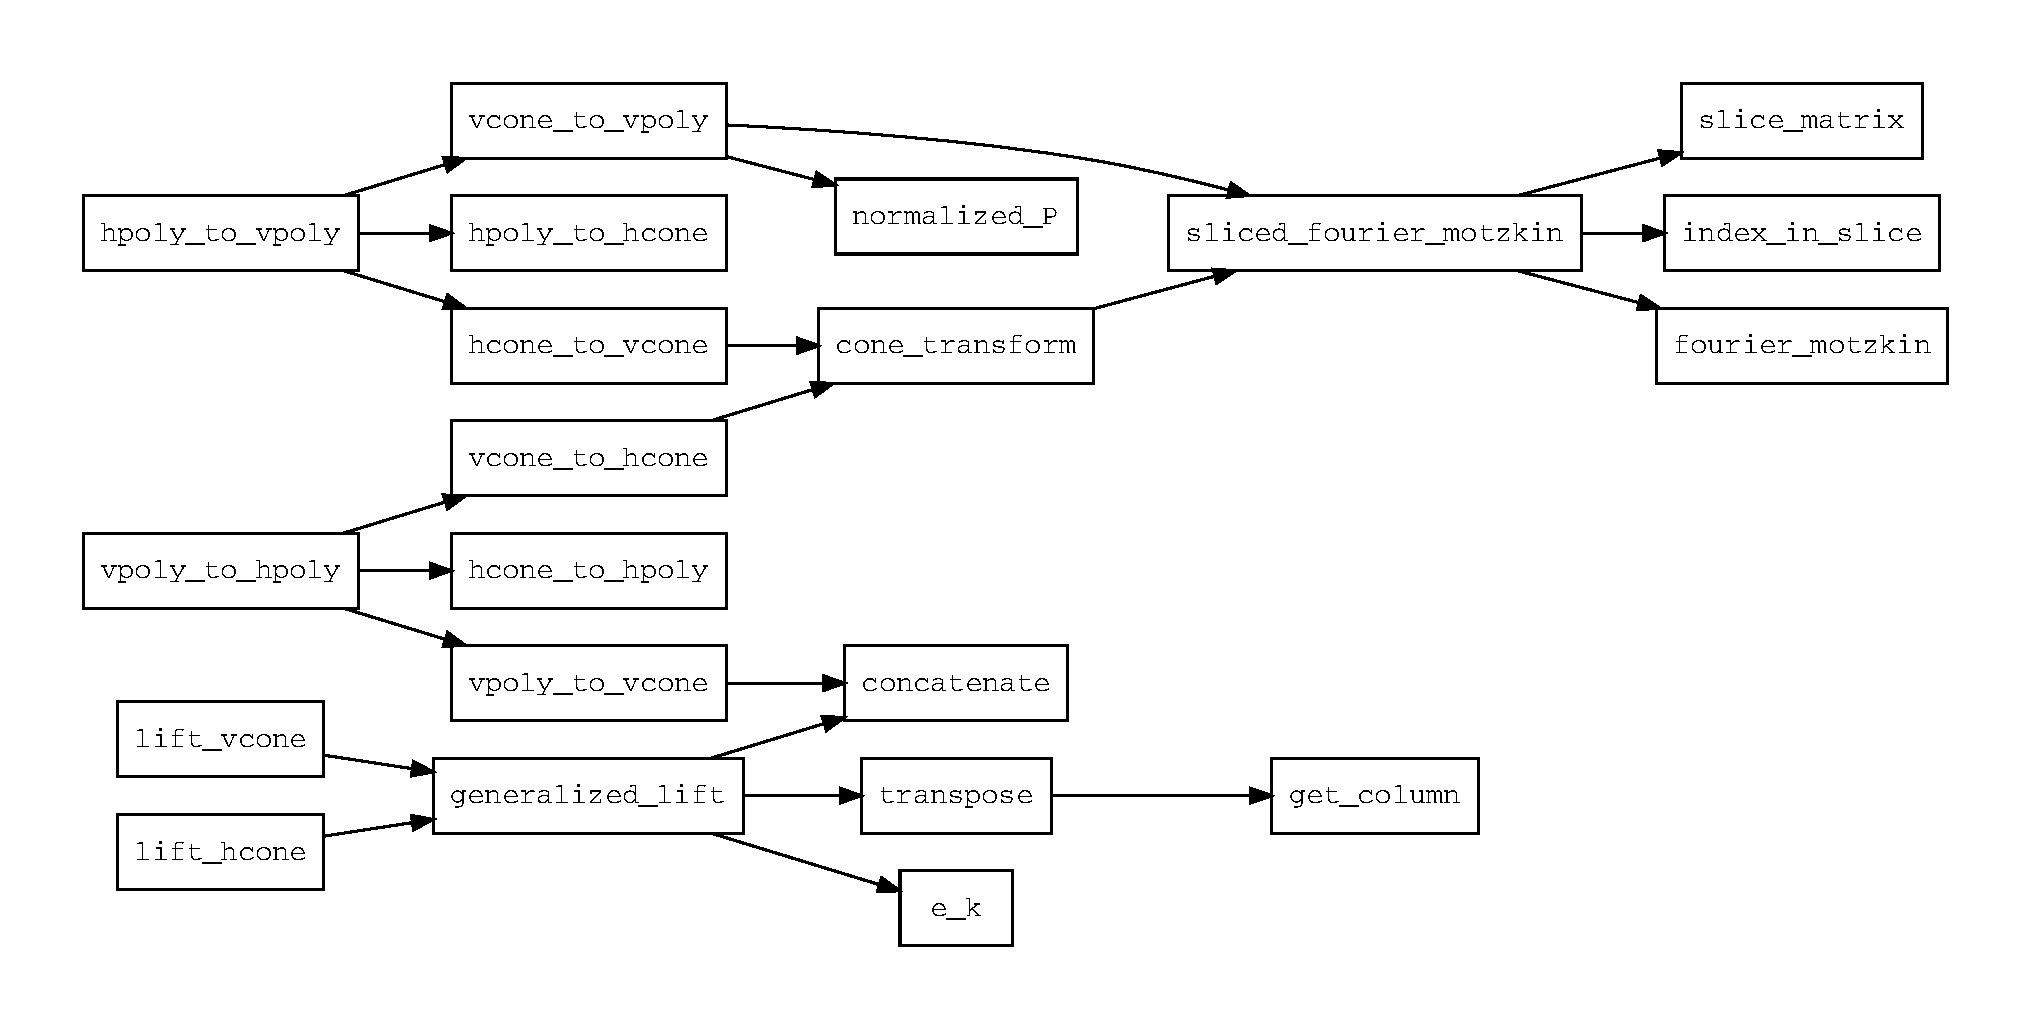
\includegraphics[angle=90, width=\textwidth]{../img/callgraph.pdf}
\end{frame}

\begin{frame}{{\tt Matrix fourier\_motzkin(Matrix,k)}}
\lstFMEPart
Partition \lsti{M} into logical sets $Z,P,N$ that satisfy the following:\\

\begin{tabular}{|l|l|l|}
	\hline
	set & range                               & property     \\
	\hline
	$Z$ & [\lsti{M.begin()}, \lsti{z_end} $)$ &
	\lsti{it} $\in Z \Leftrightarrow$ \lsti{(*it)[k]} $ = 0$ \\
	\hline
	$P$ & [\lsti{z_end}, \lsti{p_end} )       &
	\lsti{it} $\in P \Leftrightarrow$ \lsti{(*it)[k]} $ > 0$ \\
	\hline
	$N$ & [\lsti{p_end}, \lsti{M.end()})      &
	\lsti{it} $\in N \Leftrightarrow$ \lsti{(*it)[k]} $ < 0$ \\
	\hline
\end{tabular}\\
\end{frame}

\begin{frame}{{\tt Matrix fourier\_motzkin(Matrix,k)}}
\lstFMEConvolute
This function creates the sets which correspond to:

$\set{\Bik B_j - \Bjk B_i \st i \in P,\, j \in N}, \quad
	\set{\Yi Y^j - \Yj Y^i \st i \in P,\, j\in N} $
\end{frame}


\section{Pointed and Full-Dimensional Polyhedra}

\subsection{Main Results}

\begin{frame}{Pointed/ Full-Dimensional Polyhedra}
\begin{itemize}
  \item These are essentially non-degeneracy constraints.
    \begin{itemize}
      \item Pointed Polyhedra have at least one vertex
      \item Full dimensional polyhedra contain an affine independent set
    \end{itemize}

  \item Pointed V-Polyhedra and Full-Dimensional H-Polyhedra have ``essentially unique'' sets of generators
  \item These ``essentially unique'' sets make it easy to test for equivalence
  \item The characterizations are similar to ``linear independence''
\end{itemize}
\end{frame}

\begin{frame}{Testing Methods}
\begin{itemize}
  \item The basic scheme of testing is as follows:
\end{itemize}
\end{frame}

\begin{frame}{Pointed V-Cones}
\begin{itemize}
  \item The following statements are equivalent.
    \begin{enumerate}
      \item $\cone(V)$ is pointed.
      \item $\t\geq\0,\; [V\t=\0 \Rightarrow \t=\0]$
    \end{enumerate}

  \item A set $V$ is called \textit{minimal} for $\cone(V)$ if:\\
  $(\forall \vec{v} \in V)\; \cone(V\setminus\{\vec{v}\}) \subset \cone(V)$

	\item Suppose that $\cone(V)$ is pointed.  Then the following two statements are equivalent:
	\begin{enumerate}
		\item V is minimal
		\item $\t\geq\0,\,\vec{v}=V\e_i,\; [\vec{v}=V\t \Rightarrow \t=\e_i]$
	\end{enumerate}
\end{itemize}
\end{frame}

\begin{frame}{Full-Dimensional H-Cones}
\begin{itemize}
  \item All definitions are nearly identical, but we use the Farkas' lemma to consider the ``dual cone''
  \item Farkas Lemma:
    Let $U \in \R^{d\times n}$.  Precisely one of the following is true:
    \begin{align*}
       & (\exists \t \geq \0) : \x = U\t                \\
       & (\exists \y) : U^T\y \leq 0,\; \ip{\x}{\y} > 0
    \end{align*}
  \item i.e. a point is contained in a cone or can be separated from it with a hyperplane
  \item The Farkas Lemma can be used to prove the following: 
    \[\HC{A} = \HC{A'} \Leftrightarrow \cone(A^T) = \cone(A'^T)\]
    ($\cone(A^T)$ is what I call the ``dual cone'')
\end{itemize}
\end{frame}

\begin{frame}{Cones and Polyhedra}
\begin{itemize}
  \item General Polyhedra are decomposed into a ``characteristic-cone'' and polytope
  \item Suppose that $P = \HP{A}{b} = \VP{U}{V}$.  Then the following three statements are equivalent:
    \begin{enumerate}
      \item $A\vec{r}\leq\0$
      \item $(\forall \vec{x}\in P)(\forall \alpha > 0)\;\vec{x} + \alpha\vec{r} \in P$
      \item $\vec{r} \in \cone(U)$
    \end{enumerate}
  \item Note that $(2)$ in the proof above is independent of $A$ and $U$.
\end{itemize}
\end{frame}

\begin{frame}{Pointed V-Polyhedra}
\begin{itemize}
  \item In $P = \cone(U)+\conv(V)$ we need $U$ to be minimal as for V-Cones
  \item Minimality for the set $\conv(V)$ -- a polytope -- is given by the vertex set
  \item Complication: a vertex of $\conv(V)$ may not be a vertex of $P$
\end{itemize}
\end{frame}

\begin{frame}{Pointed V-Polyhedra}
\begin{itemize}
	\item If $\vec{v}$ is a vertex of $\VP{U}{V}$, then $[\vec{v} = U\vec{t} + V\blambda] \Rightarrow \vec{t} = \0$  \\
  (I call $\vec{v}$ here \textit{U-free})
  \item If $\vec{v}$ is a vertex of $\VP{U}{V}$, then $\vec{v}$ is a vertex of $\conv(V)$
	\item Let $P = \cone(U)+ \cone(V)$.  Then the following are equivalent
    \begin{enumerate}
      \item $(U,V)$ is minimal for $P$
      \item $U$ is minimal for $\cone(U)$, $V$ is the vertex set of $P$
      \item $U$ is minimal for $\cone(U)$, $V$ is the vertex set of $\conv(V)$, and $V$ is $U$-free
    \end{enumerate}

\end{itemize}
\end{frame}

\begin{frame}{Full-Dimensional H-Polyhedra}
\begin{itemize}
  \item We need another form of the Farkas Lemma:
      \[ (\exists \vec{t}\geq\0) \vec{t}^T A = \vec{y},\, \vec{t}^T\vec{b} \leq c \Leftrightarrow
        \begin{cases}
        (\forall \vec{x}) A\vec{x}\leq \0 \Rightarrow \vec{y}^T\vec{x} \leq 0 \textbf{ and } \\
        (\forall \vec{x}) A\vec{x}\leq \vec{b} \Rightarrow \vec{y}^T\vec{x} \leq c
        \end{cases}
      \]
  \item Basically, a constraint is valid for a polyhedron if and only if it is a non-negative combination of rows of constraints (plus some change)
  \item If $P = \HP{A}{\vec{b}}$ is full dimensional, and $\vec{y}^T A = \0$ with $\vec{y}\geq\0$, then either $\vec{y} = \0$ or $\vec{y}^T \vec{b} > \0$.
  \item $\vec{y}^T A = \0,\;\vec{y}^T \vec{b} > \0$ occurs when two of the bounding hyperplanes are parallel
\end{itemize}
\end{frame}

\begin{frame}{Dual Homogenization Cone}
\begin{itemize}
  \item To use minimality results, the following are used
  \item 	The following two statement are equivalent:
    \begin{enumerate}
      \item $\HP{A}{\vec{b}} = \HP{A'}{\vec{b}'}$
      \item $\cone \pmb -\vec{b}^T & -1 \\ A^T & \0 \pme = \cone \pmb -\vec{b}'^T & -1 \\ A'^T & \0 \pme$
    \end{enumerate}
  \item If $\HP{A}{\vec{b}}$ is minimal and full-dimensional, then either 
    \begin{enumerate}
      \item $\cone \pmb -\vec{b}^T & -1 \\ A^T & \0 \pme$ is minimal and pointed, or
      \item $\cone \pmb -\vec{b}^T \\ A^T \pme$ is minimal and pointed, and $\cone\pmb -\vec{b}^T \\ A^T \pme = \cone \pmb -\vec{b}^T & -1 \\ A^T & \0 \pme$
    \end{enumerate}
\end{itemize}
\end{frame}

\begin{frame}{Pointed H-Polyhedra and Full-Dimensional V-Polyhedra}
\begin{itemize}
  \item $\vec{t}$ is a non-negative vector, and abbreviate {\LI} as LI. $\bar V$ denotes $\{\vec{v}-\vec{v}'\st\vec{v},\vec{v}'\in V\}$.\\

  \renewcommand{\arraystretch}{1.3}
  \resizebox{\columnwidth}{!}{
  \begin{tabular}{|l|l|l|}\hline
          & Pointed & Full-Dimensional \\ \hline
    $\cone(U)$ & $U\vec{t}=\0 \Rightarrow \vec{t}=\0$ & $d$ LI vectors in $U$ \\  \hline
    $\cone(U)+\conv(V)$ & $U\vec{t}=\0 \Rightarrow \vec{t}=\0$ & $d$ LI vectors in $U\cup \bar V$ \\ \hline
    $\HC{A}$ & $d$ LI row vectors in $A$ & $\vec{t}^T A=\0 \Rightarrow \vec{t}= \0$ \\ \hline
    $\HP{A}{\vec{b}}$ & $d$ LI row vectors in $A$ & $\vec{t}^T A=\0 \Rightarrow \vec{t}^T\vec{b} > 0$ \\ \hline
  \end{tabular}
  }
\end{itemize}
\end{frame}

\subsection{Basic Ideas for Proofs/Implementation}

\begin{frame}{Make Titles Informative.}
\end{frame}

\begin{frame}{Make Titles Informative.}
\end{frame}

\begin{frame}{Make Titles Informative.}
\end{frame}


\section*{Summary}

\begin{frame}{Summary}

	% Keep the summary *very short*.
	\begin{itemize}
		\item
		      The \alert{first main message} of your talk in one or two lines.
		\item
		      The \alert{second main message} of your talk in one or two lines.
		\item
		      Perhaps a \alert{third message}, but not more than that.
	\end{itemize}

	% The following outlook is optional.
	\vskip0pt plus.5fill
	\begin{itemize}
		\item
		      Outlook
		      \begin{itemize}
			      \item
			            Something you haven't solved.
			      \item
			            Something else you haven't solved.
		      \end{itemize}
	\end{itemize}
\end{frame}



% All of the following is optional and typically not needed. 
\appendix
\section<presentation>*{\appendixname}
\subsection<presentation>*{For Further Reading}

\begin{frame}[allowframebreaks]
	\frametitle<presentation>{For Further Reading}

	\begin{thebibliography}{10}

		\beamertemplatebookbibitems
		% Start with overview books.

		\bibitem{Author1990}
		A.~Author.
		\newblock {\em Handbook of Everything}.
		\newblock Some Press, 1990.


		\beamertemplatearticlebibitems
		% Followed by interesting articles. Keep the list short. 

		\bibitem{Someone2000}
		S.~Someone.
		\newblock On this and that.
		\newblock {\em Journal of This and That}, 2(1):50--100,
		2000.
	\end{thebibliography}
\end{frame}

\end{document}


